%% V1.3
%% 2007/01/11
%% by Michael Shell
%% see http://www.michaelshell.org/
%% for current contact information.
%%
%% This is a skeleton file demonstrating the use of IEEEtran.cls
%% (requires IEEEtran.cls version 1.7 or later) with an IEEE journal paper.
%%
%% Support sites:
%% http://www.michaelshell.org/tex/ieeetran/
%% http://www.ctan.org/tex-archive/macros/latex/contrib/IEEEtran/
%% and
%% http://www.ieee.org/



% *** Authors should verify (and, if needed, correct) their LaTeX system  ***
% *** with the testflow diagnostic prior to trusting their LaTeX platform ***
% *** with production work. IEEE's font choices can trigger bugs that do  ***
% *** not appear when using other class files.                            ***
% The testflow support page is at:
% http://www.michaelshell.org/tex/testflow/


%%*************************************************************************
%% Legal Notice:
%% This code is offered as-is without any warranty either expressed or
%% implied; without even the implied warranty of MERCHANTABILITY or
%% FITNESS FOR A PARTICULAR PURPOSE! 
%% User assumes all risk.
%% In no event shall IEEE or any contributor to this code be liable for
%% any damages or losses, including, but not limited to, incidental,
%% consequential, or any other damages, resulting from the use or misuse
%% of any information contained here.
%%
%% All comments are the opinions of their respective authors and are not
%% necessarily endorsed by the IEEE.
%%
%% This work is distributed under the LaTeX Project Public License (LPPL)
%% ( http://www.latex-project.org/ ) version 1.3, and may be freely used,
%% distributed and modified. A copy of the LPPL, version 1.3, is included
%% in the base LaTeX documentation of all distributions of LaTeX released
%% 2003/12/01 or later.
%% Retain all contribution notices and credits.
%% ** Modified files should be clearly indicated as such, including  **
%% ** renaming them and changing author support contact information. **
%%
%% File list of work: IEEEtran.cls, IEEEtran_HOWTO.pdf, bare_adv.tex,
%%                    bare_conf.tex, bare_jrnl.tex, bare_jrnl_compsoc.tex
%%*************************************************************************

% Note that the a4paper option is mainly intended so that authors in
% countries using A4 can easily print to A4 and see how their papers will
% look in print - the typesetting of the document will not typically be
% affected with changes in paper size (but the bottom and side margins will).
% Use the testflow package mentioned above to verify correct handling of
% both paper sizes by the user's LaTeX system.
%
% Also note that the "draftcls" or "draftclsnofoot", not "draft", option
% should be used if it is desired that the figures are to be displayed in
% draft mode.
%
\documentclass[journal, ]{IEEEtran}
\usepackage{cite}
\usepackage[pdftex]{graphicx}
\usepackage[cmex10]{amsmath}
% Also, note that the amsmath package sets \interdisplaylinepenalty to 10000
% thus preventing page breaks from occurring within multiline equations. Use:
%\interdisplaylinepenalty=2500
\usepackage{algorithmic}
\usepackage{array}
\usepackage{mdwmath}
\usepackage{mdwtab}
\usepackage{eqparbox}
%\usepackage[tight,footnotesize]{subfigure}
%\usepackage[caption=false]{caption}
\usepackage[font=footnotesize]{subfig}
\usepackage{fixltx2e}
\usepackage{stfloats}
\usepackage{multirow}
\usepackage[a4paper, total={6.95in, 9.85in}]{geometry}

\ifCLASSOPTIONcaptionsoff
  \usepackage[nomarkers]{endfloat}
  \let\MYoriglatexcaption\caption
  \renewcommand{\caption}[2][\relax]{\MYoriglatexcaption[#2]{#2}}
\fi
\usepackage{url}
\usepackage{lipsum}

% *** Do not adjust lengths that control margins, column widths, etc. ***
% *** Do not use packages that alter fonts (such as pslatex).         ***

% correct bad hyphenation here
\hyphenation{op-tical net-works semi-conduc-tor}

\usepackage{etoolbox}
\begin{document}
\title{Real or Not? NLP with Disaster Tweets Project}

% author names and IEEE memberships
% note positions of commas and nonbreaking spaces ( ~ ) LaTeX will not break
% a structure at a ~ so this keeps an author's name from being broken across
% two lines.
% use \thanks{} to gain access to the first footnote area
% a separate \thanks must be used for each paragraph as LaTeX2e's \thanks
% was not built to handle multiple paragraphs
\author{Vegar~Andreas~Bergum,~\IEEEmembership{vab1g19,}
        ChangKai~Fu,~\IEEEmembership{ckf1n19,}
        Adam~Ghoumrassi,~\IEEEmembership{ag3u19,}
        PingChun~Tsai,~\IEEEmembership{pct1g19.}}
\markboth{COMP6208 Advanced Machine Learning}{}

% Reduces spacing between authors and text
\makeatletter
\patchcmd{\@maketitle}
  {\addvspace{0.5\baselineskip}\egroup}
  {\addvspace{-0.5\baselineskip}\egroup}
  {}
  {}
\makeatother

\maketitle

\begin{abstract}
This project paper discusses the use of non-neural and neural methods for binary text classification in Tweets. A range of different feature extractors, using latent semantic analysis, are tested with a wide range of models. Bayesian optimisation is used to optimise hyperparameters. Gradient Boosting with pre-trained embeddings performs best out of the non-neural methods, while a 2-layer LSTM RNN produces the best neural cross-validated result. Additionally, the BERT model is finetuned for classification, scoring better than all previous models tested. 
\end{abstract}%

\IEEEpeerreviewmaketitle

% needed in second column of first page if using \IEEEpubid
%\IEEEpubidadjcol

\section{Introduction}
\IEEEPARstart{R}{eal} or Not? NLP with Disaster Tweets is a Kaggle competition\footnote{https://www.kaggle.com/c/nlp-getting-started/overview} that provides over $7,000$ labelled tweets. This competition is a binary text classification task: are the tweets concerning a real disaster or not? Twitter is more and more being used as a real-time observational tool, according to the competition description. The motivation behind this competition is to investigate the possibilities of using Twitter as a source of monitoring for emergency services. Additionally, this competition serves as a good example of a getting-started with advanced machine learning techniques when working with highly contextual and sequential data. 

As the data is highly contextual and sequential, feature extraction becomes a crucial step in being able to accurately classify the data. This project report includes an overview of a few different latent semantic analysis techniques. Including term frequency-inverse document frequency (TF-IDF)\cite{salton1986} bag-of-words models, pre-trained word embeddings\cite{pennington2014} and self-trained character-level embeddings. With a sophisticated Bayesian optimisation approach to hyper-parameter tuning, we train and evaluate a large number of linear, non-linear and neural classifiers. Using the different feature extraction methods we compare the different classification techniques. Additionally, we investigate the use of large-scale pre-trained language models such as BERT\cite{devlin2018} to classify the tweets. 

% Just a rough suggestion
\section{Feature extraction \& latent semantic analysis}
Before conducting any sort of machine learning on text-based data, we must first convert it into a structured numerical form that can be processed by a computer. 
Latent semantic analysis\cite{dumais2004} is a technique used in natural language processing to analyse the semantic similarity between textual documents. This requires a latent space representation of tokens in the text, often at a word-level, that captures likeness in meaning. With such a representation, simple techniques like cosine angles between token-vectors can reveal similarity in semantics and contextual appearance. 

Traditionally, latent space representations were done at a document level where each dimension represents a semantic token in the document. TF-IDF is one such representation that vectorizes a document into a $v$-dimensional space, where $v$ is the size of the semantic vocabulary. The vector representation is calculated by equation \ref{eq:tfidf} for each token $t$ in a document $d$
\begin{equation}\label{eq:tfidf}
\text{tf-idf}(t, d) = \text{tf}(t, d) \times \text{idf}(t)
\end{equation}
where the inner functions are defined as
$\text{idf}(t) = \log\big[\frac{n}{\text{df}(t)}\big]+1$ and  $\text{tf}(t, d) = \log[1 + f_{t,d}]$
where $f_{t,d}$ is the number of occurrences of token $t$ in document $d$.
With this model, we have one dimension for each unique word in the vocabulary.

Other neural-based methods known as \textit{word embeddings} are widely used in many text applications or natural language processing models. GloVe \cite{pennington2014} is one such model,  which is trained in a self-supervised manner, encoding vectors based on the contextual placement of tokens in a text. This results in a vector representation where tokens that appear in similar contexts have a small cosine angle between them. 

%\begin{figure}[hbt!]
  %\centering
  %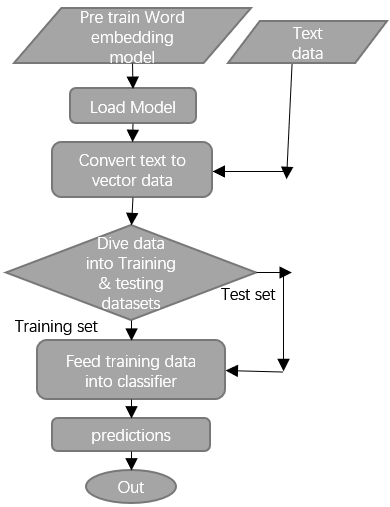
\includegraphics[ scale=0.8]{imgs/Text classification- wordembeddings2.png}
  %\caption{Text classification using word embeddings}
  %\label{fig:Work flow for Worddembeddings}
%\end{figure}

\subsection{Character Embeddings}
Tweets often incorporate highly irregular language, resulting in many words in our corpus not having a corresponding GloVe embedding. This decreases the amount of information we have available for use in the model. In an attempt to combat this, we investigated the use of character vectors instead of word vectors. As there are only a small handful of available characters, this makes it possible to have an embedding for every possible character, therefore no information is lost.

We constructed the character vectors by training a word2vec model on the Sentiment140 dataset \cite{go2009twitter}, a corpus of 1.6 million tweets, treating each individual character in a tweet as a separate token. Unfortunately, while this method was able to perform better than random guessing, the performance of this embedding type was fairly weak across all tested models, with the highest performing character embedding model having an accuracy of $66\%$. 

However, this does suggest that the character embeddings do store some useful information about the classification of the tweet, therefore, in future works, it may be beneficial to train a neural network approach that uses a combination of word and character embeddings as inputs.

In the models presented we use TF-IDF features, pre-trained GloVe word embeddings, self-trained character embeddings and BERT's built-in tokenizer.

% very niiiiice
\section{Bayesian Optimisation of Hyperparameters}
Many of the machine learning algorithms that we considered as part of this study have hyperparameters that can be adjusted to change their functionality. Constructing the optimal model for our problem requires that many combinations of these parameters be iterated over to find the parameters that allow the models to generalise best. This problem requires the use of a parameter searching strategy.

When considering how to conduct parameter search, two considerations must be taken:

Firstly, the search strategy should investigate a reasonable enough portion of the parameter space that we can be confident that we are not omitting a combination of parameters with a significantly improved performance.

Secondly, the strategy should not require excessive computation to find the optimal combination. At each iteration of the search strategy, a machine learning model will be run on our entire dataset, which uses a significant amount of both time and resources to implement. Due to our limited computing resources and pressing deadline, it would be impossible for us to perform an exhaustive search of the parameter space for each of our models.

Given these considerations, we chose Bayesian optimisation as our search strategy. This technique involves computing a probabilistic model that estimates the score of each combination of parameters in the space and iteratively updating this model by computing the output of a set of parameters if the uncertainty of this outcome is high \cite{shahriari2015taking}. Over time the optimisation model moves from “exploration” where it computes the model with parameters that it is unsure of the outcome for, to “optimisation” where it computes the model with parameters that it believes will maximise the outcome.

We ran Bayesian optimisation on each of our models using the Python package \texttt{scikit-optimise} \cite{skopt}, optimisation was conducted using $10\%$ of the data for testing and separating the remaining $90\%$ in a 80:20 split using 5-fold cross-validation and using testing accuracy as the evaluation metric. The process was initialised to run for $50$ iterations, meaning that each model would be run 250 times. As this would still take a considerable amount of time, we decided that for neural networks we would only use cross-validation on the best set of parameters dictated by the optimisation strategy, thereby requiring neural network approaches to only be run a maximum of $50$ times. Also, we implemented an early stopping strategy, whereby if the best $3$ accuracy scores of the optimisation strategy for a model were within $0.1\%$ of each other, the optimisation would be aborted as it would appear likely that this score is a ceiling past which models are unable to improve.




\begin{table*}[t]
\centering
\begin{tabular}{|l c c c c c c c c c c c c c c|} 
  \hline
   Model&Acc&$\sigma$ Acc&LSA&Depth&$\gamma$&Kernel&Optim&Hidden&\#layers&lr&Momemtum&Dropout&Filters&\#filters\\
  \hline
  CosineAngle&\textbf{0.700}&0.016&TFIDF&&&&&&&&&&&\\
  \hline
  \multirow{3}{*}{NaiveBayes}&0.573&0.025&CHAR&&&&&&&&&&&\\
  &\textbf{0.715}&0.025&GloVe&&&&&&&&&&&\\
  &0.591&0.015&TFIDF&&&&&&&&&&&\\
  \hline
  \multirow{3}{*}{GradientBoost}&0.692&0.036&TFIDF&8.0&0.0&&&&&&&&&\\
  &0.643&0.009&CHAR&5.0&0.373&&&&&&&&&\\
  &\textbf{0.789}&0.014&GloVe&3.0&0.032&&&&&&&&&\\
  \hline
  \multirow{3}{*}{RandomForest}&0.666&0.015&CHAR&8.0&&&&&&&&&&\\
  &0.583&0.04&TFIDF&6.0&&&&&&&&&&\\
  &\textbf{0.786}&0.011&GloVe&10.0&&&&&&&&&&\\
  \hline
  \multirow{3}{*}{SVM}&\textbf{0.744}&0.021&TFIDF&&0.003&Linear&&&&&&&&\\
  &0.738&0.012&TFIDF&&0.894&RBF&&&&&&&&\\
  &0.681&0.029&TFIDF&&0.077&Poly&&&&&&&&\\
  \hline
  \multirow{3}{*}{LSTM}&{\textbf{0.817}}&&GloVe&&&&Adam&100&2.0&1e4&0.99&0.268&&\\
  &0.654&&CHAR&&&&SGD&150&3.0&1e3&0.5&0.47&&\\
  &0.814&&GloVe&&&&SGD&100&2.0&1e4&0.99&0.273&&\\
  LSTM+CV&\textbf{0.801}&0.015&GloVe&&&&Adam&100&2.0&1e4&0.5&0.267&&\\
  \hline
  \multirow{3}{*}{CNN}&0.688&&CHAR&&&&Adam&&&1e3&0.5&0.351&(6,6,6)&107.0\\
  &\underline{\textbf{0.845}}&&GloVe&&&&Adam&&&1e4&0.99&0.5&(4,4,4)&150.0\\
  &0.799&&GloVe&&&&SGD&&&1e4&0.9&0.207&(3,3,3)&168.0\\
  CNN+CV&\textbf{0.799}&0.014&GloVe&&&&Adam&&&1e5&0.5&0.119&(5,4,3)&177.0\\
  \hline
  \multirow{3}{*}{BERT+CV}&\textbf{0.828}&&BERT&&&&Adam&768&12.0&5e5&&0.1&&\\
  &0.804&&BERT&&&&Adam&768&12.0&2e5&&0.1&&\\
  &0.813&&BERT&&&&Adam&768&12.0&5e5&&0.1&&\\
  \hline
\end{tabular}
\caption{Top Bayesian Optimisation Results}
\label{tab:results}
\end{table*}

\section{Data Augmentation}
The dataset supplied for this problem consists of a fairly small sample of observations, therefore, we decided that it would be useful to find a way to enrich our dataset by adding some altered samples.

To do so, we made 5 copies of each observation in the dataset, with each word in the copy having a random chance to change to a related word. The related word was chosen at random from the 5 closest words to the source word in the GloVe embedding space. This quintupled the size of our dataset.
It should be noted that we were careful to assure that the data augmentation step was only used on the training set and not the full dataset as this would result in many observations being in both the training and testing sets, thereby biasing results.
This method was tested on our CNN model and gave a minor accuracy gain of $0.5\%$. However, due to the computational complexity of our method and the relative unimportance of this addition, it was decided to omit augmentation from our official results.

\section{Non-neural methods}
To create a baseline for comparison we built a simple cosine angle similarity model based on a TF-IDF representation as described in the previous sections. The training phase consisted of building two TF-IDF corpus matrices, one for each class. In predicting the class of a new document (tweet), it was also transformed into a TF-IDF vector. Te corpus matrix with the lowest cosine angle to the new document determined the predicted class of the document. This produced a baseline scoring accuracy of exactly $70$\%, using 5-fold cross-validation. 
Table \ref{tab:results} shows a small selection of the best performing methods with a handful of feature extractor and parameter combinations. 

With this baseline, we started implementing several relevant non-neural classifiers. Firstly, a probabilistic classifier in the form of a Naive Bayes classifier. The Naive Bayes classifier uses Bayes' theorem with the independence assumption to separate the features. Even though Naive Bayes is traditionally known to work well in comparison to SVMs and other similar models with token frequency-based features, its prediction accuracies are quite low. Using both TF-IDF and the character embedding produces accuracies under $60$\%. However, with the pre-trained $200$-dimensional GloVe embeddings it beats the baseline with $1.5$ percentage points. 

To represent ensemble methods, a Gradient Boosting classifier and Random Forest classifier was trained. Table \ref{tab:results} illustrates how both methods outperform the baseline and Naive Bayes by over $8$ percentage points with the GloVe embeddings. Additionally, both outperform Naive Bayes quite drastically using the character embeddings and TF-IDF vectors. Interestingly, even though both the Random Forest and Gradient Boosting methods are based on decision trees, gradient boosting performs slightly better with a lower max-depth of the underlying trees.

The dataset only consists of $7,613$ samples. The Support Vector Machine (SVM) is known to perform well on small datasets and provides both linear and non-linear classification methods by the use of kernels. We train it using only frequency-based features (TF-IDF) and investigate three different kernels: linear, radial basis functions and polynomial. With a maximum accuracy score of $74.4$\% with the linear kernel its clearly the best performing model with the TF-IDF vectors. 

\section{Neural methods}
Utilizing deep neural methods that are capable of exploiting the sequential nature of the data will be crucial to improve upon the non-neural methods we have discussed so far. The two most commonly used architectures for this are recurrent neural networks (RNN) and convolutional neural networks (CNN). 

The best performing LSTM scores $81.7$\% accuracy using the GloVe embeddings and the Adam optimiser with a learning rate of $1.0e04$ and $0.99$ momentum. This is a 2-layer bidirectional LSTM network with a hidden dimension of $100$. The model was only trained for $6$ epochs, as the validation loss started rapidly increasing at the same time as the accuracy decreased. Even with a $26.8$\% dropout layer, it was clear that the model is very sensitive to overfitting. 
When training with 5-fold cross-validation, we get an average result of $80.1$\% accuracy, denoted LSTM+CV in table \ref{tab:results}. This is the overall best cross-validated result we were able to produce from the Bayesian optimisation routine. 

%\begin{figure}[hbt!]
  %\centering
  %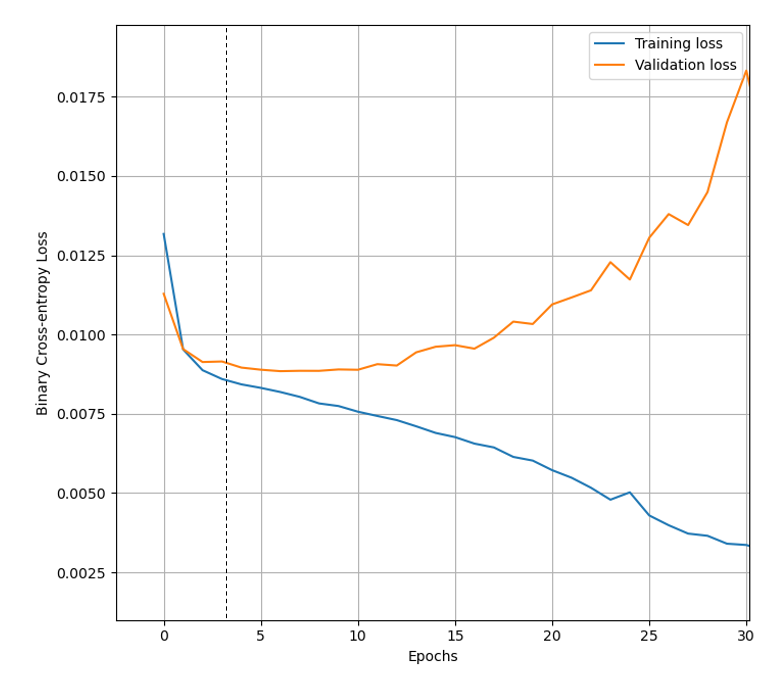
\includegraphics[width=\linewidth]{imgs/LSTM_LOSS.png}
  %\caption{LSTM-cell RNN loss during training. Training loss (blue) and validation loss (orange). Dashed vertical line indicating point of early stopping for the best performing model.}
  %\label{fig:lstm_loss}
%\end{figure}

%\begin{figure}[hbt!]
  %\centering
  %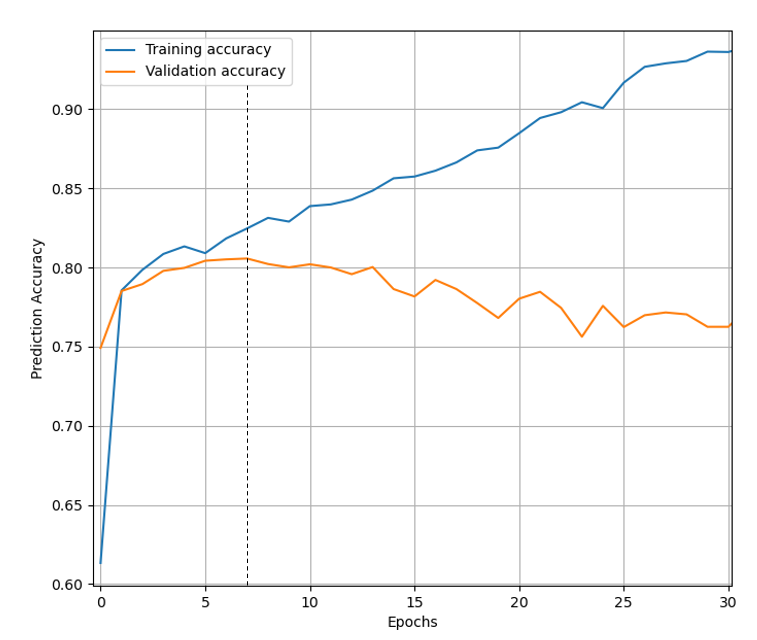
\includegraphics[width=\linewidth]{imgs/LSTM_ACC.png}
  %\caption{LSTM-cell RNN accuracy during training. Training accuracy (blue) and validation accuracy (orange). Dashed vertical line indicating point of early stopping for the best performing model.}
  %\label{fig:lstm_acc}
%\end{figure}

\begin{figure}[hbt!]
  \centering
  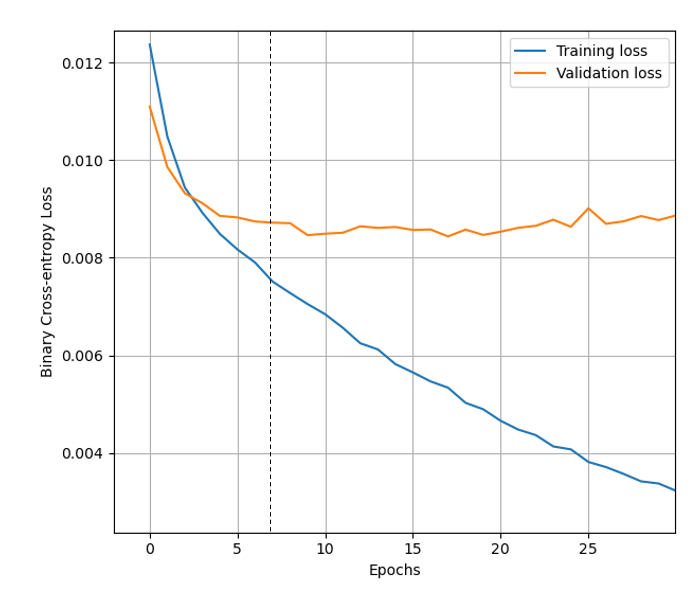
\includegraphics[width=\linewidth]{imgs/CNN_LOSS.png}
  \caption{CNN loss during training. Training loss (blue) and validation loss (orange). Dashed vertical line indicating point of early stopping for the best performing model.}
  \label{fig:cnn_loss}
\end{figure}

In addition to training the RNN, which are traditionally the best performing models on sequential data, we train a convolutional neural network. CNNs are usually used for image-based data due to its translation invariance and ability to capture spatial features. Using a kernel width that matches the embedding dimensions used, the convolutions become a sliding window across the sentence. This does, in essence, create a one-dimensional convolution over the tokens in the sentence, because the width matches the full word representation. Similarily to the RNN, figure \ref{fig:cnn_loss} illustrates the history of the loss during training. We notice that the validation loss grows rapidly after just a few epochs. Figure \ref{fig:cnn_acc} illustrates this further where we can observe that the validation accuracy decreases after just a few epochs. For brevity only the training history has been shown for the CNN - the RNN's training history is remarkably similar.
% really good :D

\begin{figure}[hbt!]
  \centering
  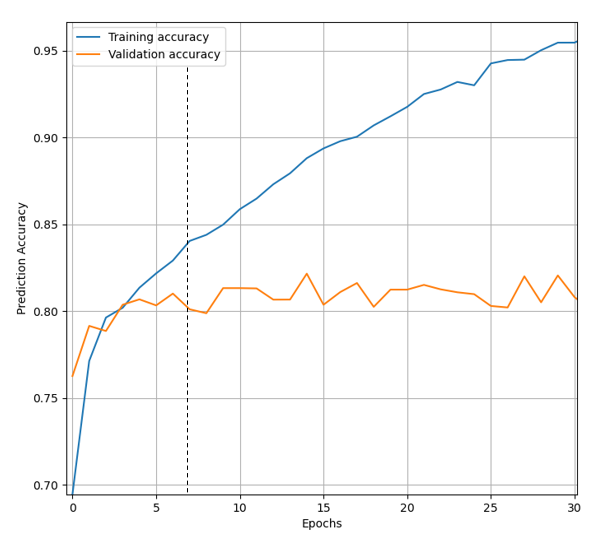
\includegraphics[width=\linewidth]{imgs/CNN_ACC.png}
  \caption{CNN accuracy during training. Training accuracy (blue) and validation accuracy (orange). Dashed vertical line indicating point of early stopping for the best performing model.}
  \label{fig:cnn_acc}
\end{figure}

The CNN ends up with a result that is within the margin of error of the LSTM's cross-validated results, at $79.9$\% accuracy (denoted CNN+CV in table \ref{tab:results}). However, a lucky non-validated training run of the CNN was able to achieve $84.5$\% test accuracy.

\section{Transfer learning}
Unlike the neural methods where the model is trained from scratch, transfer learning utilised a pre-training - fine-tuning process to gain better performance with less data. Google's BERT (Bidirectional Encoder Representations from Transformers) is probably one of the most representative pre-trained models. Firstly, BERT is trained bi-directionally to catch the embedding of each word in the sentence by feeding countless online text corpus such as Wikipedia to complete two tasks, i.e. Masked Language Model (MLM) and Next Sentence Prediction\cite{devlin2018} to gain maximum 334 million parameters. In the second phase, the model is fine-tuned through the dataset owned by the users to implement downstream tasks, such as document classification, dependency parsing, question answering and name-entity recognition. 

Since this is a binary classification NLP task, "bert-base-uncased" pre-trained model is chosen as it is built to process lower-cased English text. Its architecture has 12-layer transformers, 768 hidden and 12-heads, which means it has 110 million parameters. From figure \ref{fig:bert_acc} we could conclude that epoch 3 should be the result parameter as accuracy sharply increases at epoch 4. The best result gained is $82.8$\% accuracy using the Adam optimiser with a learning rate of $5e-5$ after $3$ epochs, which is within our expectation in the scope of transfer learning.


%\begin{figure}[hbt!]
  %\centering
  %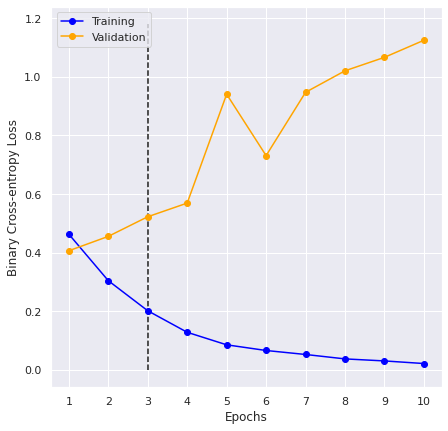
\includegraphics[width=\linewidth]{imgs/BERT_LOSS.png}
  %\caption{BERT loss during training. Training loss (blue) and validation loss (orange). The best performing model is achieved given the value of epoch is three.}
  %\label{fig:bert_acc}
%\end{figure}

\begin{figure}[hbt!]
  \centering
  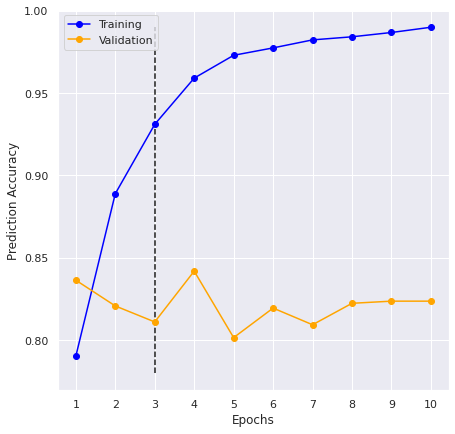
\includegraphics[width=\linewidth]{imgs/BERT_ACC.png}
  \caption{BERT accuracy during training. Training accuracy (blue) and validation accuracy (orange). The best performing model is achieved given the value of epoch is three.}
  \label{fig:bert_acc}
\end{figure}

\section{Discussion}
For the performance of feature extractors, it is obvious that the models processed by the GloVe embeddings achieve better performance than both TFIDF and character embeddings in all possible observations. In comparison, TFIDF is more reliable than character embedding in NaiveBayes and GradientBoost models, but the situation is opposite in RandomForest. This is probably due to the nature of RandomForest which makes a more precise decision with a larger amount of crucial information instead of using the frequency and inverse-frequency to represent each word.

As the training labels for the Kaggle competition were leaked, comparing our results to the leaderboard is useless. The top 50 submissions all have a perfect score of 100\% accuracy. However, by manually inspecting some of the published submissions it is clear that our best cross-validated result of $82.8$\% test accuracy is comparable. By using cross-validation and a generous validation and test-set split we can ensure that the results are representative as the models' ability are generalised. The best CNN performance at $84.5$\% could be considered an outlier as this was not reproducible in a cross-validated setting. 

\section{Conclusion}
Within our work, three feature extractors, eight models and various hyperparameters generate over 100 combinations. It is not surprising that BERT ($82.8$\% validation acc.) perform the best within these models. As expected the LSTM model catches up tightly right after at $80.1$\%. In general, the neural methods perform better than the non-neural ones with a $80$+\% threshold. It is also predictable that neural methods gain better results with reasonable deeper architectures. Although transfer learning gives a relatively easy milestone without any required pre-processing, it is still promising to investigate neural models further to see if a more reliable architecture could be created to perfectly solve critical problems such as disease classification. 

% Can use something like this to put references on a page good!
% by themselves when using endfloat and the captionsoff option.
\ifCLASSOPTIONcaptionsoff
  \newpage
\fi

% trigger a \newpage just before the given reference
% number - used to balance the columns on the last page
% adjust value as needed - may need to be readjusted if
% the document is modified later
%\IEEEtriggeratref{8}
% The "triggered" command can be changed if desired:
%\IEEEtriggercmd{\enlargethispage{-5in}}

% references section

% can use a bibliography generated by BibTeX as a .bbl file
% BibTeX documentation can be easily obtained at:
% http://www.ctan.org/tex-archive/biblio/bibtex/contrib/doc/
% The IEEEtran BibTeX style support page is at:
% http://www.michaelshell.org/tex/ieeetran/bibtex/
\bibliographystyle{IEEEtran}
% argument is your BibTeX string definitions and bibliography database(s)
%\bibliography{IEEEabrv,../bib/paper}
%
% <OR> manually copy in the resultant .bbl file
% set second argument of \begin to the number of references
% (used to reserve space for the reference number labels box)

\bibliography{references.bib}

\end{document}
